% Virtual Environment for Individual-Based Modeling - Part II
%
% Advanced Project II - Jacobs University Bremen
% Supervisor: Dr. Stefan Kettemann
%
% Created on January 10, 2019
%
% Authors:
%   Ralph Florent <r.florent@jacobs-university.de>
%   Davi Tavares <davi.tavares@leibniz-zmt.de>
%   Agostino Merico <a.merico@jacobs-university.de>
%
% - Overview
% - Features
% - Methods (Procedure)
% - Results, Discussions
% - Conclusion
% - References

% ==============================================================================
% START: Methods, Results, Discussions, Conclusion
% ==============================================================================
\section{Additional Features}\label{sec:features}
As discussed in previous sections, the first part of the project leaves a lot of rooms for improvement. As a matter of fact, that is the reason why we have decided to come up with additional features and augment the functional capabilities for both end-users and developers. Thus, we introduce in the section the set of chosen features and their importance across the application.

For the second version of the project, we have selected carefully  a set of features to gradually integrate into the first version as we maintain the same workflow scheme (see Figure \ref{fig:workflow-scheme}). These additional features are:
\begin{enumerate}
    \item \textit{File structure}
    \item \textit{More types of agents}
    \item \textit{Multiple-agent updates per processing unit}
    \item \textit{Dynamical environment.}
\end{enumerate}

\noindent
Next, we detail each one of them and their importance for the project.

\subsection{A new file structure}
Though it should not be seen as a proper\footnote{Obviously, there are many definitions of a software feature, however, this action seems more like a refactoring than a new capability to the project. Proposing a new approach for file organization is yet questionable as it does not represent a distinguishable characteristic/capability of the project.} feature for the project, yet it remains an essential factor for the refactoring of the code implementation. Renewing the file structure of the project is the first step considered before anything.

Recall that the first code implementation was done in a single Python file (basically, a Jupyter Notebook). The implementation itself was good because it follows a standard programming workflow, which implies that the code should be at least \textit{architected, standardized, structured, scalable, collaborative, documented}, and so forth \cite{rflorent2019veibm1, smashingmagazine}. However, that is not the best approach to keep up as we are adding more features and therefore increasing the degree of complexity of the project. With that being said, restructuring the file organization by breaking the main code into small chunks of code plays an important role in the project maintenance and scalability. The open source community names this decision: \say{a near-term view of implementation and a long-term vision}. Observe in the scheme below the compliant's folder and the new file structure used for the current implementation.

% Virtual Environment for Individual-Based Modeling - Part II
%
% Advanced Project II - Jacobs University Bremen
% Supervisor: Dr. Stefan Kettemann
%
% Created on January 10, 2019
%
% Authors:
%   Ralph Florent <r.florent@jacobs-university.de>
%   Davi Tavares <davi.tavares@leibniz-zmt.de>
%   Agostino Merico <a.merico@jacobs-university.de>

% ==============================================================================
% START: File Structure
% ==============================================================================

\vspace{0.6cm}
\dirtree{%
.1 <project-root>.
.2 dist.
.3 docs.pdf.
.3 \emph{...}.
.2 docs.
.3 v1.
.3 v2.
.2 graphs.
.2 samples.
.2 src.
.3 notebooks.
.4 agent.py.
.4 config.py.
.4 config.yml.
.4 constants.py.
.4 core.py.
.4 habitat.py.
.4 helpers.py.
.4 main.py.
.4 \emph{...}.
.3 tests.
.3 requirements.txt.
.3 setup.py.
.3 \emph{...}.
.2 \emph{...}.
}
\vspace{0.6cm}
% ==============================================================================
% END: File Structure
% ==============================================================================

\noindent
Being out of the scope of this document, we will not discuss here other related topics such as \textit{file structure convention, file naming, single responsibility principle}, among others. These topics are quite engaging and require further readings. Please feel free to refer to the \emph{Coding Style Guide} for Python programming at \href{https://www.python.org/dev/peps/pep-0008/}{python.org/dev/peps/pep-0008} or \href{http://google.github.io/styleguide/pyguide.html}{google.github.io/styleguide/pyguide.html} for more details.

Note that, besides the file structure, we also follow an application structure commonly called LIFT:
\begin{itemize}
    \item L: locate quickly the code
    \item I: identify the code at a glance
    \item F: keep the flattest structure possible
    \item T: try to be DRY | Don't Repeat Yourself \textit{(avoid being so DRY that it sacrifices readability).}
\end{itemize}
\noindent
Needless to say, having a good file structure along with a LIFT structure makes the project more robust and undoubtedly scalable. Now that we have a clear understanding of the file structure, let us see how we integrate the actual features with it.

\subsection{More than 2 types of agents}
In the previous version of the project, we hardcoded two (2) types of agents: \emph{short-legged} and \emph{long-legged} waterbirds. Recall as we discussed in Section \ref{sec:overview} that in the real world there are more than just two categories of waterbirds. This short- and long-legged way of categorizing the agents was a simple approach as we intend to firstly create a pilot test and then built upon it something more complex. So, based on the assumption that the belly of birds cannot touch the water because it would contradict the homeostasis theory\footnote{Birds would lose temperature rapidly.}, we involve a set of four (4) bird species, with legs sizes of 5 cm (small shorebirds), 10 cm (big shore birds), 30 cm (small herons) and 60 cm (big herons). As for their virtual representation in the VE, we discuss the implementation in Section \ref{sec:methodology}.

\subsection{Multiple-agent updates per processing unit}
Going a bit more technical, the previous implementation was lacking the functional capability of processing all the agents separately for a single update. That is to say, for $n$ processing times, only $n$ agents were randomly selected and processed\footnote{Processed: update an agent geometric position if the criteria for moving it were met.} with possibility of replacement. For instance, in a setting of 10 agents and 5 processing times, it is possible that the same exact bird gets selected and processed 5 times.

This new feature, \emph{Multiple-agent updates per processing unit}, refers to adding the capability of processing every single agent for every processing unit.

\noindent
\textbf{Important}: \textit{Be aware that we use the term \emph{process} in lieu of \emph{update} when referring to moving an agent randomly to another position. There is a little nuance and we want to keep a clear cut. It occurs that the term \emph{process} is more global and avoids the confusion that will always move. As a matter of fact, process means to try to update. An agent will move if and only if the conditions for moving to another place are met.}

\subsection{Make the environment dynamical}
Finally, we opt for using a dynamical environment, that is, by varying certain characteristics of the environment. One of the most relevant environmental factors in the VE setting is the water depth. By tweaking this parameter, we can simulate environmental changes (not in the VE though) over time and observe how the waterbirds evolve with those changes. Why? Because in real-life situations, the waterbirds' interactions and evolution are highly correlated to environmental changes.

Simulating an environment change within the virtual environment is a bit tricky and requires to tweak some variables to obtain the desired results. So, we provide more details on this specific case scenario in Section \ref{sec:methodology}.

% \subsection{Data tracking for sensitivity analysis}

\section{Methodology}\label{sec:methodology}
The methods used in the first version are still applicable for this version of the project, with the exception of employing some key changes without losing the main focus. So, we describe in the following section what has been changed and how these changes are implemented.

\subsection{The application}
What is happening now when the application runs? Recall the workflow scheme in Figure \ref{fig:workflow-scheme} that indicates the three (3) main steps \textit{Initialize, Observe, Update} used in the first part of the VE simulation. The idea is still the same, except that we include now more internal processes. As illustrated in line number \textcolor{blue}{3} of \textcolor{blue}{Listing} \ref{lst:app}, the core methods imported to operate the simulation are exactly the same. In other words, the application runs and does the following:
\begin{enumerate}
    \item first, initializes some internal configurations (we detail more about it later);
    \item next, creates $m$ number of habitats and $n$ number of agents;
    \item then, snapshots the current state of the virtual environment;
    \item then, runs the update process per time unit $t$;
    \item finally, repeat the bullet points (3) and (4) for $p$ times.
\end{enumerate}
We omit for now the \emph{post-condition} operations (scripts) since they are not part of the main idea but simply helper functionalities for future analyses.

\subsection{External configuration}
Although it implies the utilization of intensive programming to implement it, we proceed this time by adding a configuration file to load the external setup for the physical environment setting to run or simulate. The two files in charge of such a task are \emph{config.yml} and \emph{config.py} and are located under the \emph{src/notebooks} folder. For best practice and human-readability reasons \cite{mthoma2014cfgyml}, the \emph{config.yml} file is used, among other suitable options, to pass an application profile along with the parameters required by the system to operate. The profile is useful for meta operations like file system handling, for example, whereas the parameters are a way to load the core values such as habitat and/or agent information for the simulation. For example, loading dynamically the types of agents is made quite practical with the external setup. That is, an array of agents with the format shown below is expected and will be internally handled and represented as-is in the virtual environment.
\begin{minted}
    [
        baselinestretch=1.2,
        bgcolor=bg-mint,
        fontsize=\footnotesize,
    ]
    {yaml}
agents:
    - type: 30cm # unique identifier to categorize an agent
    quantity: 7  # total of agents of this kind to create
    color: '#7C79A2' # color representation of this type of agent
    label: 30cm-legged # descriptive label for the plots
    fn: # runnable function (definition, dependencies, arguments)
        def: 'lambda x: -10.89 * math.log(x) + 44.71'
        deps:
            - 'import math'
        args:
            - x
    habs: # types of habitats allowed for use
        - 1
        - 2
\end{minted}

On the other hand, the \emph{config.py} file is applied to load the main configuration in memory and apply it when it is necessary. The file serves also as basis to set some constants values as they are frequently used across the application.

\begin{listing}[H]
    \inputminted
    [
        baselinestretch=1.2, % interspace size
        bgcolor=bg-mint,
        fontsize=\footnotesize,
        linenos % show line numbers
    ]
    {python}{scripts/app.py}
    \caption{Main entry point of the application}
    \label{lst:app}
\end{listing}

\subsection{File system handling}
The initial setup involves additional settings besides loading the external configuration. These settings are the file system handling, the operating system status check, and the python environment (kernel). They help to prepare a sanitized workspace to run the application without crossing some surprising exceptions (e.g., memory leaks or overflow) at the time of execution.

The application is made smart enough to create, remove, and check the existence of files within the scope of the project. The folders \emph{samples} and \emph{graphs} are used for this purpose and contain respectively snapshots and plots files. Keep in mind that, for the file system handling, specific use cases (e.g., user permissions) are not taken into account.

\subsection{The constants}
The constants are useful when it comes to avoiding magic strings and numbers. As mentioned before, the loaded configuration is part of the constants used throughout the application. Besides that, we use constants for core elements (e.g., key identifier for the static habitats), directory and file paths, in-memory storage, and default values.

\subsection{The helpers}
As we mention in the previous sections, the core functionalities \emph{Initialize, Observe, Update} include some internal operations. For reusability reasons, we use helper functions to handle these operations such as random points generation, euclidean distance, gif maker, and so on.

\subsection{The \emph{Agent} class definition}
In the first place, the \emph{Agent} class was defined such that it accepts on-the-fly attributes. Normally, we kept it simple:
\begin{itemize}
    \item \textbf{\textit{type}}: the category name of the waterbird species;
    \item \textbf{\textit{x, y}}: the x- and y-coordinate of the agent's position within the VE.
\end{itemize}
For this implementation, we define properly the attributes for the class and add the \emph{color} and \emph{name} attributes. These represent respectively the color of an agent's specific type and a unique identifier for data tracking. Moreover, we make the \textbf{\textit{x}}- and \textbf{\textit{y}}-coordinate attributes private and combine them into a single private property called \textbf{\textit{point}} | point(x, y), a 1-dimensional tuple of shape (2,) representing a geometric position in a Cartesian plane. Being a private property, we provide the methods \emph{get\_point()} and \emph{set\_point((x, y))} acting respectively as \emph{getter} and \emph{setter} for such a property.

\subsection{The \emph{Update} algorithm}
Roughly speaking, the instructions, as referred in \textcolor{blue}{Algorithm} \ref{algo:update-ve1}, define a synchronous approach for allocating randomly a new position \emph{x, y} to an agent if the criteria for moving are met. This was the basic idea of the \emph{update} algorithm.

\vspace{0.4cm}
\begin{algorithm}[H]
    \SetAlgoLined
    \KwData{Given a randomly selected agent}
    \KwResult{Update an agent's position when doable}
    Randomly choose a new destination within an \say{acceptable} habitat\;
    Compute the probability of that new destination use for this agent \;
    \eIf{the calculated probability complies with the threshold}{
        move the selected agent to that new destination\;
    }{
       maintain the same position\;
    }
    \caption{Update (VE Part I)}
    \label{algo:update-ve1}
\end{algorithm}
\vspace{0.4cm}

Recalling that this algorithm above is defined in its most simplistic model, we had already anticipated that some changes would be necessary to make the virtual environment dynamical. As a result, to implement additional functionalities like \emph{multiple-agent update per processing unit}, we break down the general idea into 2 pieces (or callable functions): \emph{update} and \emph{update\_one}.
\begin{itemize}
    \item \textbf{\textit{update}}: (short for update all) is an iteration over all the existing agents and apply some changes;
    \item \textbf{\textit{update\_one}}: is the same \emph{update} procedure defined in \textcolor{blue}{Algorithm} \ref{algo:update-ve1}.
\end{itemize}
\noindent
\textbf{Important}: \textit{For this version of the VE prototype, we will refer to \texttt{update} as \texttt{update\_all} to avoid confusion.}

\subsection{The criteria for allocating new positions}
The criteria for allocating new positions to an agent are defined by the following characteristics: water depth, lagoon salinity, food availability, and minimal distance to human settlements. These characteristics are used to calculate the probability of moving to a new allowed destination (habitat), along with a chosen threshold\footnote{Valid for sensitivity analysis by tuning its value.}. In other words, the movement is considered adequate when the overall probability surpasses the chosen threshold.

Because of these criteria, we use internally a set of helpers to compute specific operations like the minimal distance to the human settlements, for example. Observe the lines \textcolor{blue}{22, 23, 24, 35} in \textcolor{blue}{Listing} \ref{lst:update-one} the respective helper functions \emph{gen\_rand\_point(), which\_habitat(), compute\_dist(), eval\_fn()}. Keep in mind that the calculations in lines \textcolor{blue}{36, 37, 38} are statically set, and therefore, overly apply to any type of agents. That is because the specific functions for these probability calculations are still missing.

\begin{listing}[H]
    \inputminted
    [
        baselinestretch=1.2, % interspace size
        bgcolor=bg-mint,
        fontsize=\footnotesize,
        linenos % show line numbers
    ]
    {python}{scripts/update-one.py}
    \caption{Update agent in one unit of time}
    \label{lst:update-one}
\end{listing}

\section{Results \& Discussions}
To test out the second version of the VE prototype, we prepare a setting with these values shown in Table \ref{table:test-setting}. Obviously, this setting is configured using the YAML file, \emph{config.yml}, which, in turn, is loaded via the \emph{config.py} for future use.

\begin{table}[!ht]
    \begin{center}
        \begin{tabular}{ ||l|l|l|| }
            \hline
            \multicolumn{3}{ ||c|| }{ \textbf{Setting for Testing}} \\
            \hline \hline
            \textbf{\textit{Processing times}} & \multicolumn{2}{c||}{25} \\
            \hline
            \textbf{\textit{Threshold}} & \multicolumn{2}{c||}{$1 * e^{-7}$}\\
            \hline
            \multirow{4}{*}{\textbf{\textit{Waterbirds species}}}& 5 cm & 5 in Habitat 1 \\\cline{2-3}
            & 10cm & 4 in Habitat 1\\\cline{2-3}
            & 30cm & 7 in Habitat 1, 2\\\cline{2-3}
            & 60cm & 5 in Habitat 1, 2, 3\\\cline{2-3}
            \hline
            \multirow{4}{*}{\textbf{\textit{Rainfall distribution}}}& time: 1-10 & 20 units \\\cline{2-3}
            & time: 11-20 & 200 units\\\cline{2-3}
            & time: 21-30 & 600 units\\\cline{2-3}
            & time: 31-40 & 30 units\\\cline{2-3}
            & time: 41-50 & 0 \\
            \hline
        \end{tabular}
        \caption{Values and parameters used to load the configuration for the initial setup of the VE prototype. The results are shaped in accordance with these preset values, but not necessarily the same due to the randomness the initial state.}
        \label{table:test-setting}
    \end{center}
\end{table}

Note that there is no external configuration format for the habitats yet. That is because the code implementation is tightly coupled to the existing design (and geometry) initially set. Automating the design setting for the VE prototype would add more complexity to the current virtual environment, hence, it can be tackled down in a future release of the prototype. Similarly, be aware that the specific probability functions used to compute the overall probability of moving an agent are not normalized yet. That is the reasons why the chosen threshold is so relatively low. Otherwise, the agent would never get updated. Fair tuning values for the threshold should be in the range of two (2) decimals (e.g., 0.10; 0.25; 0.50, etc.).

The feature, \emph{multiple-agent updates per processing unit}, makes the VE computations expensive and time-consuming. Given the handheld device\footnote{Laptop with limited computational resources (RAM + CPU).} used to try out the setting, we choose a considerably fair processing times value, which is twenty-five (25) to run our tests. That is, for a total number of twenty-one (21) agents, the \emph{update\_one} function will be executed $21 * 25$ times. That is just the tip of the iceberg. Deep down within the \emph{update\_one()} function is the \emph{gen\_rand\_one()} called to generate a randomly \say{acceptable} position. Depending on the habitat's capacity, this \emph{gen\_rand\_one()} function can be quite time- and memory-consuming due to its infinite search for new positions.


Now that we have explained the reasons of our values and parameters choices, let us present the obtained results that correspond to the chosen setting.
\begin{figure}[!ht]
    \centering
    \frame{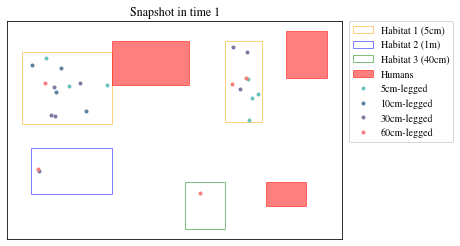
\includegraphics[width=\textwidth]{results/sample.png}}
    \caption{Example of a snapshot sample. Taken at the very first processing time, this snapshot displays the physical environment setting and distribution of agents within the simulation.}
    \label{fig:snapshot-sample}
\end{figure}

In Figure \ref{fig:snapshot-sample}, we present an example of a snapshot when running the VE simulation. This snapshot is taken in time 1 during the execution, which is the initial state of the components within the VE. Then, for every processing unit, a new snapshot will be generated and saved. Recall that this preview illustrated in Figure \ref{fig:snapshot-sample} is simply a visual aid for observations. But, in reality, we use a dictionary-based data format to hold in memory a summary of each state after processing, which is later on used for other purposes such as generating plots, data tracking, and sensitivity analysis.

The graph shown in Figure \ref{fig:graph-distribution} is actually a graphical representation of that summary mentioned above. For example, each subplot displays the distribution of the waterbirds' frequency in each lagoon.
\begin{figure}[!ht]
    \centering
    \frame{\includegraphics[width=\textwidth]{results/graph.pdf}}
    \caption{Summary of the simulation of the waterbirds in the tropics. This simulation corresponds to the setting used in Table \ref{table:test-setting}.}
    \label{fig:graph-distribution}
\end{figure}

Despite the new changes brought up to this version of the simulation, there is still room for improvement. Roughly speaking, we can enumerate the following flaws:
\begin{itemize}
    \item the units need to be double-checked and standardized;
    \item the probability functions need to be double-checked and normalized;
    \item the real-world values must mapped correctly the values used in the virtual environment;
    \item the habitats' capacity are not taken into account, yet it remains an essential criterion for moving;
    \item the current code implementation is not unit-tested;
    \item the application is partially documented;
    \item among other considerations.
\end{itemize}

\clearpage
\newpage
\section{Conclusion}
In this document, the main changes performed on the first version of the virtual environment have been highlighted and described. These changes are the main aspects that characterize the second version of this project. This version of the simulation is technically more robust and partly automated through external configurations.

This VE prototype is now capable of simulating a dynamical environment along with different waterbirds species. Meanwhile, it lacks some implementation regarding the probability functions that are specific to the waterbird species and the characteristics (salinity, food) of the given physical environment.

A test setting is chosen to try out the core functionalities of the prototype. The simulation works as expected and the test results surely prove it. Unfortunately, no conclusion concerning the waterbirds' evolution or interactions can be drawn yet as the assumptions from the coastal lagoons are still in their analysis stage.
% ==============================================================================
% END: Methods, Results, Discussions, Conclusion
% ==============================================================================